\documentclass[laboratorio]{guia}

\def \practnum {2}
\def \practica {Ley de Ohm y de Kirchhoff}
% \def \practica {Circuitos el\'{e}ctricos de corriente continua}

\def \materia {Laboratorio de F\'\i sica II para Qu\'\i micos}
\def \periodo {2do. Cuatrimestre de 2015}
\def \catedra {Pablo Cobelli}
\def \website {http://materias.df.uba.ar/f2qa2015c2}
 
\usepackage{graphics}
\usepackage{amsmath}
\usepackage{amsfonts}
\usepackage{graphicx}
\usepackage{float}
\usepackage{wrapfig}
\usepackage{subfigure}
\usepackage{bm}
\usepackage{grffile}
\usepackage{color}
\usepackage{framed}
\usepackage[utf8]{inputenc}
\usepackage[T1]{fontenc}
\usepackage{lmodern}
\usepackage{circuitikz}
\usepackage[spanish]{babel}
\usepackage{babelbib}
\selectbiblanguage{spanish}

 

%----------------------------------------------------------
% Agrega al path de figuras el subdirectorio con el mismo
%     nombre que el archivo principal del proyecto
\graphicspath{{./\jobname/}}

%----------------------------------------------------------
% Definicion del entorno 'sabermas'
\makeatletter
\definecolor{shadecolor}{rgb}{0.89,0.91,0.94}
\newenvironment{sabermas}[1]{%
\vfill
\begin{shaded}
  \begin{center}
  {\textsection{Para saber m\'as}}
  \end{center}
  #1
\sf } 
{%
\end{shaded}%
}
\makeatother

%----------------------------------------------------------
% Definicion del entorno 'problema'
\newcounter{ContadorProblema}
\setcounter{ContadorProblema}{0}
\newcounter{TieneFiguraAsociada}
\setcounter{TieneFiguraAsociada}{0}
\newcounter{UbicacionFigura}
\setcounter{UbicacionFigura}{0}

\newenvironment{problema}[2][]
{%
    \ifx\relax#1\relax%
        \setcounter{TieneFiguraAsociada}{0}
        \else
        \setcounter{TieneFiguraAsociada}{1}
    \fi
    \def \archivofigura {#1}
    % 
    \refstepcounter{ContadorProblema}
    \noindent%
    \ifnum\value{TieneFiguraAsociada} < 1%
        {\sffamily \bfseries Problema \arabic{ContadorProblema}.}
        %{\sc {#1}}%
        \par\nobreak\par\nobreak%
        \medskip 
    \else
        % Va con figura; resta determinar de que lado.
        \ifnum\value{UbicacionFigura} < 1
            % Poner la figura del lado derecho
            \begin{minipage}{12.25cm}
            {\sffamily \bfseries Problema \arabic{ContadorProblema}.}
            %{\sc {#1}}%
            \par\nobreak\par\nobreak%
            \medskip 
        \else
            % Poner la figura del lado izquierdo
            \begin{minipage}{4.5cm}
                \centering
                \includegraphics[width=4.5cm]{\archivofigura}
                {\footnotesize {\sffamily Esquema asociado al 
                problema \arabic{ContadorProblema}}.}
            \end{minipage}\hfill%
            \begin{minipage}{12.25cm}
                {\sffamily \bfseries Problema \arabic{ContadorProblema}.}
                %{\sc {#1}}%
                \par\nobreak\par\nobreak%
                \medskip 
        \fi
    \fi
}
{%
    \ifnum\value{TieneFiguraAsociada} < 1%
        % \par \bigskip \vskip 0.3cm
    \else
        % Va con figura; resta determinar de que lado.
        \ifnum\value{UbicacionFigura} < 1
            % Poner la figura del lado derecho
            \end{minipage}\hfill%
            \begin{minipage}{4.5cm}
                \centering
                \includegraphics[width=4.5cm]{\archivofigura}
                {\footnotesize {\sffamily Esquema asociado al 
                problema \arabic{ContadorProblema}}.}
            \end{minipage}
        \else
            % Poner la figura del lado izquierdo
            \end{minipage}%
        \fi
    \fi
    \setcounter{TieneFiguraAsociada}{0}
    \par \bigskip \vskip 0.3cm
    % Permutamos el valor de la ubicacion
    \ifnum\value{UbicacionFigura} < 1
        \setcounter{UbicacionFigura}{1}
    \else
        \setcounter{UbicacionFigura}{0}
    \fi
}

%----------------------------------------------------------
% Definicion/Redefinicion de estilos
\renewcommand{\vec}[1]{\ensuremath{\mathbf{#1}}}



\hyphenation{ coe-fi-cien-tes coe-fi-cien-te au-to-va-lor
              au-to-va-lo-res co-rres-pon-der pro-ble-ma 
              cual-quie-ra po-la-ri-za-cio-nes }

\graphicspath{{./Guia_Ohm/}}

\begin{document} 
\objetivo{
    Investigar la dependencia entre corriente y diferencia de potencial eléctrica en diversos dispositivos eléctricos.
	% Estudiar distintos métodos de medición de resistencias: a) usando voltímetros y amperímetros, b) usando óhmetros.
	Verificar leyes de Kirchhoff y el teorema de Thévenin.
	\tematicas{Ley de Ohm, leyes de Kirchhoff, teorema de Thévenin.}
	} 
\maketitle

\section{Corriente en función de la diferencia de potencial}
Se propone observar la dependencia de la corriente \(I\) que atraviesa una
resistencia \(R\) al variar la diferencia de potencial \(\Delta V\) aplicada a la misma.
Se usarán amperímetros y voltímetros para medir estas magnitudes físicas.
Se propone realizar el estudio en los siguientes casos:
\begin{enumerate}
\item En el circuito de la figura \ref{fig:1} se muestra una resistencia \(R\) conectada a una fuente que provee un valor de diferencia de potencial constante en el tiempo, más conocida como fuente de continua.
Mida y grafique la dependencia de \(I\) en función distintos valores que puede asumir una resistencia variable.
Para determinar el valor de esta última, no se fíe de la indicación del perillero de la caja de resistencias, use en su defecto la función óhmetro de un multímetro.
¿Cómo comparan las \(\Delta V\) obtenidas sobre la resistencia, también llamada caída de tensión o simplemente tensión, con la fuerza electromotriz \(\varepsilon_0\) entregada por la fuente?

\item El circuito de la figura \ref{fig:2} hace uso de una fuente de continua, una resistencia variable \(R_1\) y otra fija que llamaremos resistencia de carga \(R_2\).
Se busca medir y graficar la dependencia de la(\(\Delta V\)) sobre \(R_2\) en función de la \(I\) que la atraviesa.
Para determinar esta última, ¿dónde debe ubicar un amperímetro?
¿Qué relación encontró entre las variables medidas?
¿Qué obtiene de tal relación aritmética?
Observación: el conjunto de una fuente fija de tensión continua y una resistencia variable es equivalente a tener una fuente de tensión variable.
Este tipo de circuito se llama \emph{divisor resistivo} y presenta una tensión de salida \(\Delta V= \frac{R_2}{R_1+ R_2} \varepsilon_0\).

\item Reemplazar en el circuito de la figura \ref{fig:2} la resistencia de carga por una lámpara de filamento incandescente.
Medir y graficar la dependencia de \(\Delta V\) sobre la lámpara en función de \(I\).
Describa la relación entre \(I\) y \(\Delta V\), y trate de explicar qué está sucediendo.
Puesto que el filamento empieza a ``iluminarse'' para \(\sim \SI{12}{\volt}\) realice varias mediciones por encima y debajo de esa \(\Delta V\).
\end{enumerate}

\begin{figure}[t!]
    \centering
	\begin{circuitikz}
		\draw
		to [short, -*] (3,0) 
		to [short] (0,0) 
		to [battery1, l=\(\varepsilon_0\)] (0,2) 
		to [ammeter, i=\(I\)] (3,2) 
		to [short, *-] (5,2)
		% node[anchor=west]{B}
		(3,2) to [R, l=\(R\)] (3,0) 
		(5,0) to [short] (3,0)
        (5,2 )to[voltmeter,color=white,name=M](5,0);
        \mymeter{M}{0}  % try 90, 0, -90
		;
	\end{circuitikz}
    \caption{Circuito básico para la medición de diferencia de potencial \(\Delta V\), y corriente \(I\) sobre una resistencia \(R\).}
    \label{fig:1}
\end{figure}

%\begin{figure}[t!]
%    \centering
%    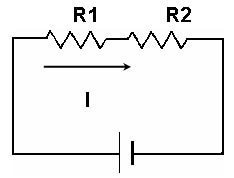
\includegraphics[width=8.5cm]{LG02--002.png}
%    \caption{Circuito básico para la medición de diferencia de potencial \(\Delta V\), y corriente \(I\) sobre una resistencia \(R\).}
%    \label{fig:2}
%\end{figure}

\begin{figure}[t!]
    \centering
	\begin{circuitikz}
		\draw
		(5,0) node[above=15]{\(\Delta V\)}
		to [short, o-*] (3,0) 
		to [short] (0,0) 
		to [battery1, l=\(\varepsilon_0\)] (0,3) 
		to [short] (3,3) 
		% node[anchor=west]{B}
		(3,3) to [R, l=\(R_1\)] (3,1.5) 
		(3,1.5) to [R, l=\(R_2\)] (3,0) 
		(3,1.5) to [short, *-o] (5,1.5)
		;
	\end{circuitikz}
    \caption{
		Fuente que provee una diferencia de potencial variable \(\Delta V\), a partir de una fija \(\varepsilon_0\).
	}
    \label{fig:2}
\end{figure}

%\begin{figure}[t!]
%    \centering
%    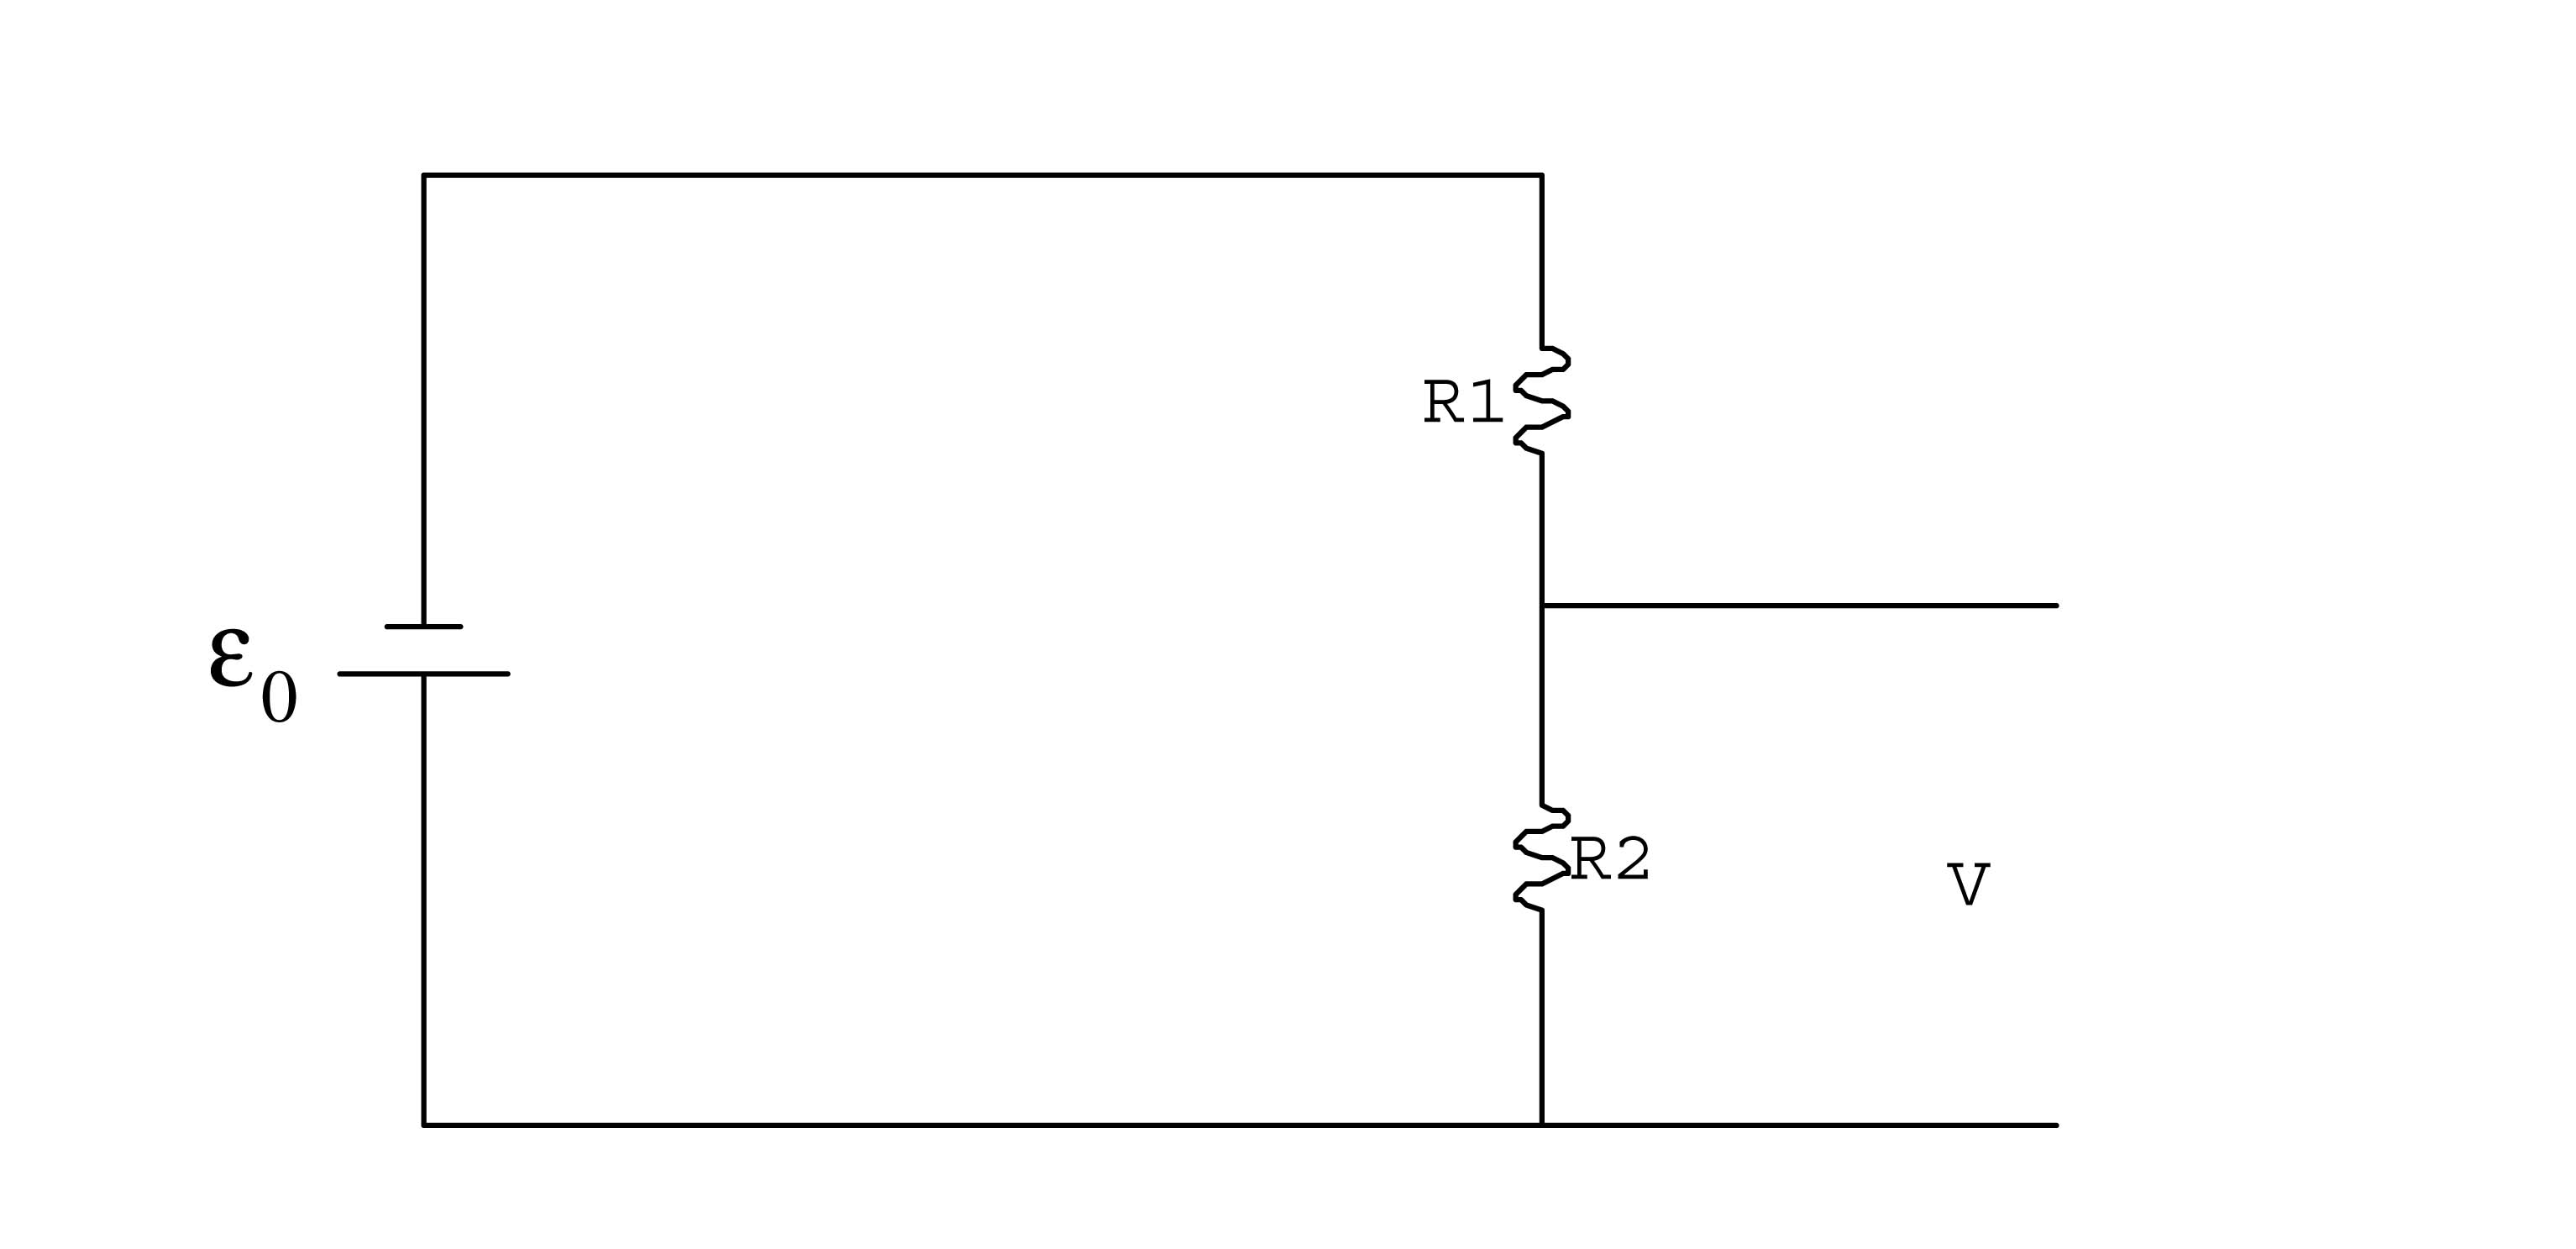
\includegraphics[width=8.5cm]{LG02--001.png}
%    \caption{
%		Fuente que provee una diferencia de potencial variable \(\Delta V\), a partir de una fija \(\varepsilon_0\).
%	}
%    \label{fig:2}
%\end{figure}


\section{Leyes de Kirchhoff}
El físico alemán Gustav Kirchhoff describió en 1845 dos leyes que relacionan corrientes y diferencias de potencial en circuitos eléctricos.
\begin{description}
	\item{1"a ley:} La suma de las intensidades que se dirigen hacia un nodo es igual a la suma de las corrientes que abandonan dicho nodo (un nodo es el punto de confluencia de tres o más conductores).
	\item{2"a ley:} La suma de las caídas de tensión o diferencias de potencial a lo largo de un circuito cerrado es nula.
\end{description}

\begin{figure}[t!]
    \centering
	\begin{circuitikz}
		\draw
		(0,0) to [R, i=\(I\), l=\(R_1\)] (2.5,0)
		(2.5,0) to [R, l=\(R_2\)] (5,0)
		to [short] (5,-1.5)
		to [battery1, l=\(\varepsilon_0\)] (0,-1.5) 
		to [short] (0,0)
		;
	\end{circuitikz}
	\begin{circuitikz}
		\draw
		(0,-1) to [R, i=\(I_2\), l=\(R_2\), *-*] (5,-1)
		(0,0) to [R, i=\(I_1\), l=\(R_1\)] (5,0)
		% (0,0) to [R, i=\(I_1\), v=\(\Delta V_2\) l=\(R_1\)] (5,0)
		to [short] (5,-2)
		to [battery1, l=\(\varepsilon_0\)] (0,-2) 
		to [short, i=\(I\)] (0,-1)
		to [short] (0,0)
		;
	\end{circuitikz}
    \caption{Circuito serie (arriba) y paralelo	(debajo).}
    \label{fig:3}
\end{figure}

%\begin{figure}[t!]
%    \centering
%    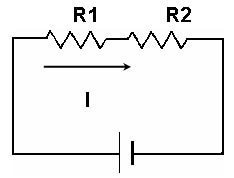
\includegraphics[width=0.25\textwidth]{LG02--002.png}
%    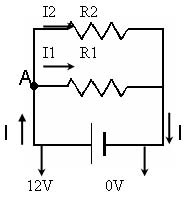
\includegraphics[width=0.25\textwidth]{LG02--003.png}
%    \caption{
%		Circuito serie (arriba) y paralelo	(debajo).
%	}
%    \label{fig:3a}
%\end{figure}
En la figura \ref{fig:3} se presentan conexiones de resistencias en serie y paralelo.
Verifique el cumplimiento de las leyes de Kirchhoff.


\section{Teorema de Thévenin}
Una característica importante de toda fuente de tensión es su resistencia interna.
Por ejemplo, si tenemos una batería cuyo voltaje de terminal es \(\varepsilon_0\) cuando por ella no pasa corriente, es decir, cuando no se está tomando potencia de la misma, el voltaje que mediremos cuando la fuente esté conectada a un circuito que sí tome potencia variará dependiendo de cuánta corriente circule por ella.
En general, una fuente de tensión está formada por circuitos eléctricos o electrónicos complejos, sin embargo para todos los fines prácticos es posible suponer que la fuente de tensión real está formada por una fuente ideal de tensión \(\varepsilon_\mathrm{th}\) y una resistencia en serie \(R_\mathrm{th}\), también llamada la resistencia interna de la fuente.
Esta última afirmación es el enunciado de un teorema muy útil de la teoría de circuitos llamado \emph{Teorema de Thévenin}. 

\begin{figure}[t!]
    \centering
	    \begin{circuitikz}
		\draw (-.2,3.5) node{Fuente}; 
        \draw[dotted] (-1.2,-.25) -- (.8,-.25) -- (.8,3.25) -- (-1.2,3.25) -- cycle;
        % \draw[loosely dotted] (-1.2,-.25) -- (.8,-.25) -- (.8,3.25) -- (-1.2,3.25) -- cycle;
        \draw
		(5,0) to [short, -*] (3,0)
		(0,0) to [ammeter] (3.5,0)
        (0,0) to [R, l=\(R_\mathrm{th}\)] (0,1.5)
		to [battery1, l=\(\varepsilon_\mathrm{th}\)] (0,3)
        to [short, i=\(I\), -*] (3,3)
        to [short] (5,3)
        (3,3) to [R, l=\(R\)] (3,0)
		to [short] (5,0)
		to[voltmeter,color=white,name=M](5,3);
		\mymeter{M}{0}  % try 90, 0, -90
        ;
	\end{circuitikz}
	% 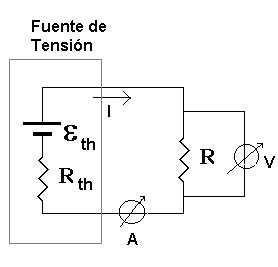
\includegraphics[width=7.5cm]{LG02--004.png}
    \caption{
		Circuito para determinar la resistencia interna de la fuente \(R_\mathrm{th}\), y la diferencia de potencial teórica que entregaría en vacío \(\varepsilon_\mathrm{th}\).
	}
    \label{fig:4}
\end{figure}

El objeto de esta actividad es verificar en un caso práctico la validez del teorema de Thévenin y determinar la resistencia interna de una fuente de tensión.
Se propone armar el circuito que se indica esquemáticamente en la figura \ref{fig:4}.
Para ello se requiere de una resistencia variable \(R\), un amperímetro y un voltímetro.
Asegúrese de que la resistencia externa \(R\) pueda disipar la potencia eléctrica cuando se le aplique la máxima tensión, y para ello estime la \(I_\mathrm{m\acute{a}x}\) que pasará por la misma (utilizando el valor mínimo de la resistencia) y la potencia máxima asociada.

Según el teorema de Thévenin, para el circuito de la figura \ref{fig:4} se tiene
\begin{equation}
	\Delta V_\mathrm{R}= \varepsilon_\mathrm{th}- I R_\mathrm{th},
\end{equation}
donde \(\Delta V_\mathrm{R}\) es la diferencia de potencial medida por el voltímetro conectado a la resistencia \(R\) e \(I\) la corriente medida por el amperímetro.

El experimento propuesto consiste en variar \(R\) y para cada valor de la misma medir \(\Delta V_\mathrm{R}\) e \(I\).
Luego grafique estos valores.
De ser válido el enunciado del teorema de Thévenin, tal gráfico debe evidenciar una respuesta lineal, en la que la pendiente determina \(R_\mathrm{th}\) y la ordenada al origen el valor de \(\varepsilon_\mathrm{th}\).
Verifique entonces la validez del teorema de Thévenin en todo el rango que pueda explorar de \(I\) y haga su propia estimación de la resistencia interna de la fuente.
Como \(R_\mathrm{th}\) incluye la resistencia interna del amperímetro \(R_\mathrm{A}\) debe consultar la documentación de este instrumento para poder calcular la de la fuente.

\nocite{Alonso1998,Purcell1988}
% \nocite{Alonso1998,Purcell1988,Reitz1996,Trelles1984,Reitz1996}
\bibliographystyle{unsrt} 
\bibliography{Bibliografia}

\end{document}
